\section{Protocol Background}\label{sec:background}

USD.AI issues two tokens on Arbitrum, its hub chain~\cite{usdaidocs}. \emph{USDai} is minted one-for-one against approved stablecoins (PYUSD, M\textsuperscript{0}'s wM and USDC over our window) by KYC'd institutions through \texttt{deposit()} and burned back to a stablecoin through \texttt{withdraw()}. It does not accrue yield. \emph{sUSDai} is a vault over USDai. Deposits are synchronous under ERC-4626~\cite{eip4626}. Exits are asynchronous under ERC-7540~\cite{eip7540}: a holder calls \texttt{requestRedeem()}, which burns the shares and joins a first-in, first-out queue. An administrator role then services the queue at fixed windows (the documentation gives 30 days as an example) by calling \texttt{serviceRedemptions()}. The vault prices deposits at an \emph{optimistic} NAV and redemptions at a \emph{conservative} NAV, and the two coincide only when no loans are active~\cite{usdaidocs}.

Vault capital reaches borrowers through a lending stack (Fig.~\ref{fig:arch}). The vault commits USDai to a deposit or escrow timelock keyed by a \texttt{loanTermsHash}. A \emph{Loan Router} originates the loan, mints lender position NFTs, and routes monthly repayments of principal and interest back to tranche lenders. Collateral is a wrapped bundle of GPU-backed tokens, and loans are non-recourse to the borrower's parent except for ``bad acts''~\cite{usdaidocs}. A second yield source, a \emph{Base Yield Escrow}, holds PYUSD issuer incentives that are periodically harvested into the vault as newly minted USDai. Earlier in our window, yield on M\textsuperscript{0}'s wM reserve was also minted into the vault as base yield. Both tokens are bridged with LayerZero burn-and-mint OFTs~\cite{layerzero} to Ethereum, Base, Plasma and Solana. Every core contract can be paused by an administrator role, and operations are submitted by a multisig~\cite{usdaidocs}.

The source code and its full git history are public~\cite{usdaisrc}. We use them in two places. First, every event signature we decode comes from that code, including signatures that were later renamed or removed. Second, the history shows a V1 to V2 Loan Router upgrade (commit \texttt{43dd6d5}, 2026-05-29) and a temporary \texttt{migrateLoan()} path, which we see executed on-chain between 2026-06-26 and 2026-07-14.

\begin{figure}[t]
\centering
\resizebox{\columnwidth}{!}{% Protocol architecture as measured in this study (Fig. 1).
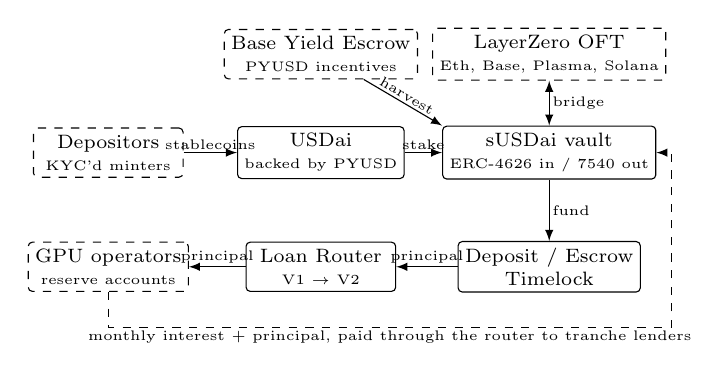
\begin{tikzpicture}[
  font=\scriptsize, >=latex,
  box/.style={draw, rounded corners=1.5pt, align=center, inner sep=2.5pt, minimum height=6mm, minimum width=19mm, fill=white},
  ext/.style={box, dashed},
  lab/.style={font=\tiny, align=center, inner sep=1pt}]
  % row 1
  \node[ext] (dep)   at (0,0)    {Depositors\\{\tiny KYC'd minters}};
  \node[box] (usdai) at (2.7,0)  {USDai\\{\tiny backed by PYUSD}};
  \node[box] (vault) at (5.6,0)  {sUSDai vault\\{\tiny ERC-4626 in / 7540 out}};
  \node[ext] (lz)    at (5.6,1.25) {LayerZero OFT\\{\tiny Eth, Base, Plasma, Solana}};
  \node[ext] (bye)   at (2.7,1.25) {Base Yield Escrow\\{\tiny PYUSD incentives}};
  % row 2
  \node[box] (dt)    at (5.6,-1.45) {Deposit / Escrow\\Timelock};
  \node[box] (lr)    at (2.7,-1.45) {Loan Router\\{\tiny V1 $\rightarrow$ V2}};
  \node[ext] (bor)   at (0,-1.45)   {GPU operators\\{\tiny reserve accounts}};
  % flows
  \draw[->] (dep) -- node[lab, above] {stablecoins} (usdai);
  \draw[->] (usdai) -- node[lab, above] {stake} (vault);
  \draw[<->] (vault) -- node[lab, right] {bridge} (lz);
  \draw[->] (bye) -- node[lab, above, sloped] {harvest} (vault.north west);
  \draw[->] (vault) -- node[lab, right] {fund} (dt);
  \draw[->] (dt) -- node[lab, above] {principal} (lr);
  \draw[->] (lr) -- node[lab, above] {principal} (bor);
  \draw[->, dashed] (bor.south) -- ++(0,-0.45) -- node[lab, below] {monthly interest + principal, paid through the router to tranche lenders} ++(7.15,0) |- (vault.east);
\end{tikzpicture}
}
\caption{USD.AI as reconstructed in this study. Solid arrows are flows we measure directly from Arbitrum event logs. Dashed boxes are parties or venues whose internal state is not on the hub chain.}
\label{fig:arch}
\end{figure}

\section{Data and Methodology}\label{sec:method}

\subsection{Data acquisition}
All chain data comes from the Covalent GoldRush REST API~\cite{goldrush} (Table~\ref{tab:data}). The study window runs from the vault's deployment block (Arbitrum block 335{,}730{,}936, \StudyStart{}) to block \EndBlock{} (\StudyEnd{}). The first vault deposit, and so the first NAV observation, is on 2025-05-14. Livepeer and Akash are measured over the same dates. We pull three kinds of data:
\begin{itemize}
\item \textbf{Complete transaction histories}, with decoded logs, for the nine lending-stack contracts (Table~\ref{tab:data}).
\item \textbf{Event scans} of the USDai and sUSDai contracts for 15 event types. The topic endpoint accepts at most $10^6$ blocks per call, so the window is split into 182 non-overlapping block windows. Windows that are fully in the past are cached; the open window is always refetched.
\item \textbf{Snapshots}: current holders of USDai and sUSDai on four chains, and daily USD prices.
\end{itemize}
We also use the weekly median H100 on-demand rental price from a frozen GetDeploying snapshot (CC~BY~4.0)~\cite{getdeploying}, the same file used in~\cite{cerron2026gpu}. Its SHA-256 matches the original.

\begin{table*}[t]
\caption{Data sources and what each one supplies}
\label{tab:data}
\centering
\small
\renewcommand{\arraystretch}{1.25}
\begin{tabular}{@{}l l p{9.2cm}@{}}
\toprule
\textbf{Source} & \textbf{Endpoint or method} & \textbf{What we pull} \\
\midrule
GoldRush & \texttt{transactions\_v3} & Full decoded history of the 9 lending contracts: Loan Router V1 and V2, deposit, escrow and collateral timelocks, reserve-account factory, collateral wrapper, base yield escrow \\
GoldRush & \texttt{events/topics} & 15 vault and USDai event types over 182 block windows; Livepeer \texttt{TicketBroker} ticket payments \\
GoldRush & \texttt{token\_holders\_v2} & Current holders of USDai and sUSDai on 4 chains; monthly sUSDai holders on Ethereum at past blocks \\
GoldRush & \texttt{historical\_by\_addresses\_v2} & Daily market prices of sUSDai, USDai, PYUSD and WETH \\
GoldRush & \texttt{transactions\_summary} & Activity of top holders and borrowers \\
GoldRush & \texttt{address/\{a\}/activity} & Every chain each borrower and top holder has used \\
GoldRush & \texttt{balances\_v2} & Current holdings of traced wallets \\
\midrule
Arbitrum node & \texttt{eth\_call} & Vault accounting views at one block \\
Arbitrum node & \texttt{eth\_getLogs} & Independent re-pull of every event set, to check GoldRush (Section~\ref{sec:verify}) \\
Arbitrum node & \texttt{tokenURI}, \texttt{ownerOf} & Hardware-token metadata links and holders for every pledged token \\
USD.AI metadata host & HTTPS & The protocol's own record for each hardware token: model, units, stated value, useful life \\
Solana node & \texttt{getTokenSupply} & sUSDai and USDai supply on Solana \\
Akash Console API & REST & Akash spend, leased GPUs, providers, GPU prices \\
GetDeploying & frozen file & Weekly median H100 rental price (CC BY 4.0) \\
\bottomrule
\end{tabular}
\end{table*}

\subsection{Decoding}
We decode raw logs ourselves rather than rely on third-party ABI coverage. For each event we compute $\textit{topic}_0=\mathrm{keccak256}(\textit{signature})$ from the published source. A log is accepted only if its topic count matches the number of indexed parameters, which, for example, rejects ERC-721 \texttt{Transfer} events. The data field is then ABI-decoded. V2 originations, migrations and refinancings carry the full \texttt{LoanTermsV2} struct: borrower, currency, collateral token IDs, tranche lenders, amounts and per-second rates, repayment schedule and fee specifications. We decode it to recover terms that V1 only kept in calldata. The decoder recognizes \EventsDecoded{} events. Two topic hashes on the V1 router match no signature in the repository history; we count them and exclude them.

\subsection{Stitching the loan book}
A loan changes identity when it is migrated or refinanced, because each event retires one \texttt{loanTermsHash} and creates another. We build a forest in which each new hash points to its predecessor and resolve every repayment to the root origination. Migrated loans name a per-borrower \emph{reserve account} as the new borrower. The factory event \texttt{ReserveAccountCreated(account, borrower)} maps each reserve account back to the underlying borrower. Each hash keeps the currency of its own terms: V1 loans were denominated in PYUSD or USDC (6 decimals) and migrated loans in USDai (18 decimals). Outstanding principal is the principal of the current terms minus principal repaid under those terms. The tranche rate $r$ is per-second and scaled by $10^{18}$, so the annual rate is $\mathrm{APR}=r\cdot 31{,}536{,}000/10^{18}$. Loans below \$1{,}000 are test loans and are excluded.

\subsection{Vault accounting}
Let $\mathcal{D}_d$ be the set of sUSDai \texttt{Deposit} events on day $d$. We define the deposit-side NAV and the global share supply as
\begin{align}
\mathrm{NAV}_d &= \operatorname{median}_{e\in\mathcal{D}_d}\frac{\mathit{assets}_e}{\mathit{shares}_e},\\
S_d &= \sum_{e\le d}\mathit{shares}^{\text{mint}}_e-\sum_{e\le d}\mathit{shares}^{\text{request}}_e .
\end{align}
NAV is forward-filled on days without deposits. Shares are burned when a redemption is requested, not when it is paid. Bridging moves shares between chains without changing $S_d$; we validate $S_d$ against the sum of the four holder snapshots. The yield accrued to holders in a period $P$ is
\begin{equation}
Y_P=\sum_{d\in P} S_{d-1}\,(\mathrm{NAV}_d-\mathrm{NAV}_{d-1}),
\end{equation}
and the cash that reached the vault is $C_P=I_P+B_P+F_P+E_P$. Here $I_P$ is loan interest paid to the vault (\texttt{LenderRepaid} with the vault as lender), $B_P$ is base yield harvested into the vault, $F_P$ is fees paid to the vault, and $E_P$ is escrow interest credited on escrow withdrawal or cancellation, net of the 10\% router admin fee. The \emph{cash coverage ratio} $\kappa=C/Y$ asks how much of the NAV growth holders were credited with arrived as cash. A ratio below one means part of the reported yield is accrued, not received. That is normal for loans that pay monthly, but it should close over time.

\subsection{Holders, queue and GPU prices}
For each chain we report holder count, top-$k$ shares, the Herfindahl-Hirschman index (HHI) and the Gini coefficient. Top holders are labeled using the contract metadata names GoldRush returns for logs they emit. Redemption requests are matched to \texttt{RedemptionProcessed} events by request ID to obtain wait times and pending shares. Finally, we compute Spearman's $\rho$ between weekly requested shares and the H100 rental price, both its level and its week-over-week change. The sample is small, so this is descriptive and not causal.

\subsection{Reconciliation with on-chain state}
Event-derived numbers can be wrong in ways that are hard to see from the events alone. We therefore read the vault's own accounting views (\texttt{totalAssets}, \texttt{totalShares}, \texttt{bridgedSupply}, \texttt{depositTimelockBalance}, \texttt{loanRouterBalances}, the deposit and redemption share prices, and related views) with \texttt{eth\_call} at a single Arbitrum block, \StateBlock{}. GoldRush does not expose arbitrary contract calls, so this one step uses the public Arbitrum RPC. Every reconciliation in Section~\ref{sec:recon} compares an independently computed event total to one of these views.

\subsection{Following escrowed funds}
The vault can commit USDai to an escrow timelock against a \texttt{loanTermsHash} before any loan with that hash exists. When an escrow deposit has no matching origination, we follow the stablecoins. Starting from the escrow facility that received the USDai, we pull complete transaction histories with GoldRush and decode every ERC-20 \texttt{Transfer} of USDai, PYUSD and USDC, plus USDai \texttt{Withdrawn} events, which mark redemption of USDai into PYUSD. We expand two hops and stop at wallets with more than 1{,}500 transactions, which we treat as services. We label wallets only by their on-chain role. We do not attribute them to off-chain entities.

\subsection{Decentralized compute markets}
To put GPU credit next to realized on-chain demand for compute, we measure two live markets. \emph{Livepeer} pays for video transcoding and AI inference with probabilistic micropayments on Arbitrum. A gateway funds a deposit in the \texttt{TicketBroker} contract and an orchestrator redeems winning tickets. Each \texttt{WinningTicketTransfer(sender, recipient, amount)} event is ETH that actually moved from a payer to a provider. We scan it over the same window and price it at the daily WETH price from GoldRush. \emph{Akash} runs on its own Cosmos chain, which GoldRush does not index. We take its daily USD spend, active GPU count, provider count and per-model GPU prices from the public Akash Console API, and label them as such. Finally, we compare GPU rental prices on Akash with the centralized-cloud H100 median in the GetDeploying snapshot.

\subsection{Where each number comes from}
Event logs, transaction histories, holder lists, prices, cross-chain activity and wallet balances come from GoldRush. The vault's accounting views at one block come from \texttt{eth\_call} on a public Arbitrum node, Solana token supply from a public Solana node, Akash figures from the Akash Console API, and GPU rental prices from GetDeploying. Section~\ref{sec:verify} re-checks the GoldRush event data against a public node.

\subsection{Reproducibility}
Raw responses are canonicalized into \texttt{data/frozen} with a SHA-256 manifest. \texttt{reproduce.py} regenerates every number, table and figure in this paper offline; numbers enter the text through generated \LaTeX{} macros. The repository has 40 unit tests, including tests that the API key cannot leak, and runs them in CI.
